\chapter{Реализация}

Реализация игры разделена на несколько модулей, как и описано выше. 

Ссылку на листинги программы см. в приложениях.

\section{Используемые технологии}

Создание движка будет вестись на языке С++. Это мощный и  популярный язык для разработки настольных приложений.

Разработка будет вестись в среде CLion от компании JetBrains. Она также является популярной, имеет широкий набор возможностей. Кроме того, производитель предоставляет бесплатные лицензии учащимся. 

Компилятором является GNU G++ 12.2, а системой сборки --- CMake 3.26. Они оба имеют открытый исходный код и бесплатны. Проект создан при помощи дополнения cmake-init.

Для управления терминальным выводом используется библиотека rang[6].

В \texttt{main()} содержится основная логика программы: инициализация игры, получение ходов, их применение, обнаружение шахов. Всё остальное расположено в классах программы.

\section{Классы}

\subsection*{Класс Bitboard}

Как уже было сказано, этот класс построен на основе \texttt{std::bitset}. Он имеет следующие основные методы:
\begin{description}
	\item[\texttt{test}] проверяет, является ли бит единицей
	\item[\texttt{set}] делает бит единицей
	\item[\texttt{reset}] делает бит нулём
	\item[\texttt{count}] считает количество единиц
	\item[\texttt{find\_first}] ищет первую единицу
	\item[\texttt{find\_last}] ищет последнюю единицу
\end{description}

Они в основном полагаются на уже встроенные методы \texttt{std::bitset}, кроме \texttt{find\_first} и \texttt{find\_last}: они используют скан-таблицу[5].

Имеются также некоторые вспомогательные методы (битовых операций и ввода-вывода).

Отметим, что нумерация битов начинается со старшего (most significant) бита. Тогда получится такое соответствие квадратам доски (табл. \ref{tab: accord}):

\begin{table}[h]
	\centering
	\caption{Соответствие}
	\label{tab: accord}
	\begin{tabular}{|l|l|l|l|l|l|l|l|l|}
		\hline
		& A & B  & C  & D  & E  & F  & G  & H  \\ \hline
		8 & 0 & 8  & 16 & 24 & 32 & 40 & 48 & 56 \\ \hline
		7 & 1 & 9  & 17 & 25 & 33 & 41 & 49 & 57 \\ \hline
		6 & 2 & 10 & 18 & 26 & 34 & 42 & 50 & 58 \\ \hline
		5 & 3 & 11 & 19 & 27 & 35 & 43 & 51 & 59 \\ \hline
		4 & 4 & 12 & 20 & 28 & 36 & 44 & 52 & 60 \\ \hline
		3 & 5 & 13 & 21 & 29 & 37 & 45 & 53 & 61 \\ \hline
		2 & 6 & 14 & 22 & 30 & 38 & 46 & 54 & 62 \\ \hline
		1 & 7 & 15 & 23 & 31 & 39 & 47 & 55 & 63 \\ \hline
	\end{tabular}
\end{table}

\subsection*{Класс Board}

Также реализует сказанное выше: 12 битовых досок на каждый тип фигур каждого цвета, 2 на сторону, 2 на пустые клетки сторон, доски для занятых и свободных клеток. 

Метод \texttt{update} обновляет вспомогательные доски и вызывается после каждой модификации.

При создании принимает FEN-строку. Тут каждой фигуре соостветствует своя буква: p для пешки (pawn), r для ладьи (rook), n для коня (knight), b для слона (bishop), q для ферзя (queen), k для короля (king). Цвет определяется регистром буквы: прописные --- белые, строчные --- черные.

\subsection*{Класс Hash}

Реализация хеширования (содержит поле с хешем доски). Использует заранее сгенерированные генератором константы для обозначения фигур на позициях, добавляя или удаляя при вызове функции \texttt{put\_piece}. При этом используется тождество $a\oplus a = 0$.

\subsection*{Класс Move}

Экземпляры этого класса хранят в себе ход. Он содержит несколько полей (откуда, куда, тип и цвет фигуры, съеденную фигуру, флаги продвижения). 

\subsection*{Класс RecentHistory}

Экземпляры этого класса содержит в себе историю последних ходов. Это нужно для реализации правила 3-х ходов. Строится на основе \texttt{std::unordered\_map}. Позволяет узнавать количество повторов по хешу позиции. Очищается при взятии или продвижении.

\subsection*{Класс Position}

Экземпляры класса хранят текущую позицию: доску, счетчики ходов, хеш, историю ходов. 

Основной метод --- \texttt{apply\_move}: применяет ход, описываемый в классе Move.

Инициализация происходит при помощи FEN-строки.

\subsection*{Класс PseudoLegalMoveMaskGen}

Этот класс генерирует битовые маски движения для всех фигур, с учетом правил ходов (кроме шахов и других подобных). Отдельно генерируются взятия пешками. К сожалению, в этом классе есть несколько не очень эффективных методов, однако, это не сильно влияет на производительность.

Здесь же находится функция \texttt{in\_danger}, проверяющая, не бьётся ли какая-либо фигура другими. Для этого генерируются все маски из данной позиции и проверяется, не находятся ли там фигуры, которые могут съесть данную.

\subsection*{Класс MoveList}

Экземпляры этого класса хранят в себе список возможных ходов от генератора. В остальном схож с массивом (имеет методы \texttt{[]}, \texttt{push\_back}, \texttt{size}).

\subsection*{Класс LegalMoveGen}

Этот класс генерирует ходы на основе ранее созданных масок. Делается это так: из маски при помощи \texttt{find\_last} достается следующий ход. Он проверяется на правильность (король не окажется под ударом) и записывается в список ходов \texttt{MoveList}. Имеется возможность генерировать только взятия.

\subsection*{Класс Static}

Этот класс реализует оценку позиции как было сказано выше. Для получения оценки вызывается функция \texttt{evaluate}.

Итоговые цены для фигур получились как в табл. \ref{tab: material} [6].

\begin{table}[h]
	\centering
	\caption{Цена фигуры}
	\label{tab: material}
	\begin{tabular}{|l|l|l|l|l|l|l|l|l|}
		\hline
		Фигура & Цена \\ \hline
		Пешка & 100 \\ \hline
		Конь & 300 \\ \hline
		Слон & 350  \\ \hline
		Ладья & 500 \\ \hline
		Ферзь & 900 \\ \hline
	\end{tabular}
\end{table}

Считается, что Король имеет очень большое значение; здесь же это просто не учитывается.

А цена за каждое битое поле этими фигурами представлена в табл. \ref{tab: mobility}.

\begin{table}[h]
	\centering
	\caption{Цена фигуры}
	\label{tab: mobility}
	\begin{tabular}{|l|l|l|l|l|l|l|l|l|}
		\hline
		Фигура & Цена \\ 
		\hline
		Конь & 9 \\ 
		\hline
		Слон & 4  \\ 
		\hline
		Ладья & 3 \\ 
		\hline
		Ферзь & 3 \\ 
		\hline
	\end{tabular}
\end{table}

\subsection*{Класс Human}

Это интерфейс взаимодействия игрока и игры (т.е. получения от него хода). Считывается ход игрока (в формате \textbf{e2e3}, откуда (\textbf{е2}) --- куда(\textbf{е3})). Если ход содержит продвижение, то спрашивается, какое именно: нужно указать букву фигуры.

\subsection*{Класс AI}

В этом классе содержится вышеупомянутый алгоритм поиска.  Однако здесь имеются некоторые интересные особенности.

Алгоритм альфа-бета запускается в отдельном потоке --- так можно настроить время (а значит и глубину) поиска; также пользователю не будет казаться, что программа <<зависла>>. По истечении времени взводится флаг остановки, и поиск прекращается. Возвращаемое значение --- оценка и ход.

Он состоит из двух частей: минимизирующей (для черных) и максимизирующей (для белых).

Циклом жестко задаётся глубина основного поиска (она постепенно наращивается). Когда алгоритм достигает этой глубины, запускается алгоритм оценки.

Время можно регулировать снизу и сверху.

Оба предыдущих класса содержат метод \texttt{getMove}, при помощи которого программа получает от них ход.

\section{Итог разработки}

Был создан движок для монгольских шахмат. Ввод-вывод получился терминальным, и интерфейс выглядит вот так: 

\begin{figure}[h]
	\centering
	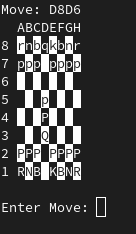
\includegraphics[width=0.25\textwidth]{interface}
	\caption{Интерфейс}
	\label{fig: interface}
\end{figure}